\documentclass[twoside]{book}

% Packages required by doxygen
\usepackage{calc}
\usepackage{doxygen}
\usepackage{graphicx}
\usepackage[utf8]{inputenc}
\usepackage{makeidx}
\usepackage{multicol}
\usepackage{multirow}
\usepackage{textcomp}
\usepackage[table]{xcolor}

% Font selection
\usepackage[T1]{fontenc}
\usepackage{mathptmx}
\usepackage[scaled=.90]{helvet}
\usepackage{courier}
\usepackage{amssymb}
\usepackage{sectsty}
\renewcommand{\familydefault}{\sfdefault}
\allsectionsfont{%
  \fontseries{bc}\selectfont%
  \color{darkgray}%
}
\renewcommand{\DoxyLabelFont}{%
  \fontseries{bc}\selectfont%
  \color{darkgray}%
}

% Page & text layout
\usepackage{geometry}
\geometry{%
  a4paper,%
  top=2.5cm,%
  bottom=2.5cm,%
  left=2.5cm,%
  right=2.5cm%
}
\tolerance=750
\hfuzz=15pt
\hbadness=750
\setlength{\emergencystretch}{15pt}
\setlength{\parindent}{0cm}
\setlength{\parskip}{0.2cm}
\makeatletter
\renewcommand{\paragraph}{%
  \@startsection{paragraph}{4}{0ex}{-1.0ex}{1.0ex}{%
    \normalfont\normalsize\bfseries\SS@parafont%
  }%
}
\renewcommand{\subparagraph}{%
  \@startsection{subparagraph}{5}{0ex}{-1.0ex}{1.0ex}{%
    \normalfont\normalsize\bfseries\SS@subparafont%
  }%
}
\makeatother

% Headers & footers
\usepackage{fancyhdr}
\pagestyle{fancyplain}
\fancyhead[LE]{\fancyplain{}{\bfseries\thepage}}
\fancyhead[CE]{\fancyplain{}{}}
\fancyhead[RE]{\fancyplain{}{\bfseries\leftmark}}
\fancyhead[LO]{\fancyplain{}{\bfseries\rightmark}}
\fancyhead[CO]{\fancyplain{}{}}
\fancyhead[RO]{\fancyplain{}{\bfseries\thepage}}
\fancyfoot[LE]{\fancyplain{}{}}
\fancyfoot[CE]{\fancyplain{}{}}
\fancyfoot[RE]{\fancyplain{}{\bfseries\scriptsize Generated on Fri Jun 20 2014 18\-:23\-:29 for Ph2\-\_\-\-Hw\-Interface by Doxygen }}
\fancyfoot[LO]{\fancyplain{}{\bfseries\scriptsize Generated on Fri Jun 20 2014 18\-:23\-:29 for Ph2\-\_\-\-Hw\-Interface by Doxygen }}
\fancyfoot[CO]{\fancyplain{}{}}
\fancyfoot[RO]{\fancyplain{}{}}
\renewcommand{\footrulewidth}{0.4pt}
\renewcommand{\chaptermark}[1]{%
  \markboth{#1}{}%
}
\renewcommand{\sectionmark}[1]{%
  \markright{\thesection\ #1}%
}

% Indices & bibliography
\usepackage{natbib}
\usepackage[titles]{tocloft}
\setcounter{tocdepth}{3}
\setcounter{secnumdepth}{5}
\makeindex

% Hyperlinks (required, but should be loaded last)
\usepackage{ifpdf}
\ifpdf
  \usepackage[pdftex,pagebackref=true]{hyperref}
\else
  \usepackage[ps2pdf,pagebackref=true]{hyperref}
\fi
\hypersetup{%
  colorlinks=true,%
  linkcolor=blue,%
  citecolor=blue,%
  unicode%
}

% Custom commands
\newcommand{\clearemptydoublepage}{%
  \newpage{\pagestyle{empty}\cleardoublepage}%
}


%===== C O N T E N T S =====

\begin{document}

% Titlepage & ToC
\hypersetup{pageanchor=false}
\pagenumbering{roman}
\begin{titlepage}
\vspace*{7cm}
\begin{center}%
{\Large Ph2\-\_\-\-Hw\-Interface \\[1ex]\large 1.\-1 }\\
\vspace*{1cm}
{\large Generated by Doxygen 1.8.5}\\
\vspace*{0.5cm}
{\small Fri Jun 20 2014 18:23:29}\\
\end{center}
\end{titlepage}
\clearemptydoublepage
\tableofcontents
\clearemptydoublepage
\pagenumbering{arabic}
\hypersetup{pageanchor=true}

%--- Begin generated contents ---
\chapter{Namespace Index}
\section{Namespace List}
Here is a list of all namespaces with brief descriptions\-:\begin{DoxyCompactList}
\item\contentsline{section}{\hyperlink{namespace_ph2___hw_description}{Ph2\-\_\-\-Hw\-Description} }{\pageref{namespace_ph2___hw_description}}{}
\item\contentsline{section}{\hyperlink{namespace_ph2___hw_interface}{Ph2\-\_\-\-Hw\-Interface} }{\pageref{namespace_ph2___hw_interface}}{}
\end{DoxyCompactList}

\chapter{Hierarchical Index}
\section{Class Hierarchy}
This inheritance list is sorted roughly, but not completely, alphabetically\-:\begin{DoxyCompactList}
\item \contentsline{section}{Ph2\-\_\-\-Hw\-Description\-:\-:Be\-Board}{\pageref{class_ph2___hw_description_1_1_be_board}}{}
\begin{DoxyCompactList}
\item \contentsline{section}{Ph2\-\_\-\-Hw\-Description\-:\-:Glib}{\pageref{class_ph2___hw_description_1_1_glib}}{}
\end{DoxyCompactList}
\item \contentsline{section}{Ph2\-\_\-\-Hw\-Description\-:\-:Cbc\-Comparer}{\pageref{struct_ph2___hw_description_1_1_cbc_comparer}}{}
\item \contentsline{section}{Ph2\-\_\-\-Hw\-Description\-:\-:Cbc\-Reg\-Item}{\pageref{struct_ph2___hw_description_1_1_cbc_reg_item}}{}
\item \contentsline{section}{Ph2\-\_\-\-Hw\-Interface\-:\-:Data}{\pageref{class_ph2___hw_interface_1_1_data}}{}
\item \contentsline{section}{Ph2\-\_\-\-Hw\-Interface\-:\-:Event}{\pageref{class_ph2___hw_interface_1_1_event}}{}
\item exception\begin{DoxyCompactList}
\item \contentsline{section}{Ph2\-\_\-\-Hw\-Interface\-:\-:Exception}{\pageref{class_ph2___hw_interface_1_1_exception}}{}
\end{DoxyCompactList}
\item \contentsline{section}{Ph2\-\_\-\-Hw\-Description\-:\-:Front\-End\-Description}{\pageref{class_ph2___hw_description_1_1_front_end_description}}{}
\begin{DoxyCompactList}
\item \contentsline{section}{Ph2\-\_\-\-Hw\-Description\-:\-:Cbc}{\pageref{class_ph2___hw_description_1_1_cbc}}{}
\item \contentsline{section}{Ph2\-\_\-\-Hw\-Description\-:\-:Module}{\pageref{class_ph2___hw_description_1_1_module}}{}
\end{DoxyCompactList}
\item \contentsline{section}{Ph2\-\_\-\-Hw\-Interface\-:\-:Reg\-Manager}{\pageref{class_ph2___hw_interface_1_1_reg_manager}}{}
\begin{DoxyCompactList}
\item \contentsline{section}{Ph2\-\_\-\-Hw\-Interface\-:\-:Be\-Board\-Interface}{\pageref{class_ph2___hw_interface_1_1_be_board_interface}}{}
\item \contentsline{section}{Ph2\-\_\-\-Hw\-Interface\-:\-:Cbc\-Interface}{\pageref{class_ph2___hw_interface_1_1_cbc_interface}}{}
\item \contentsline{section}{Ph2\-\_\-\-Hw\-Interface\-:\-:Glib\-Interface}{\pageref{class_ph2___hw_interface_1_1_glib_interface}}{}
\end{DoxyCompactList}
\end{DoxyCompactList}

\chapter{Data Structure Index}
\section{Class List}
Here are the classes, structs, unions and interfaces with brief descriptions\-:\begin{DoxyCompactList}
\item\contentsline{section}{\hyperlink{class_interface_1_1_h_w_interface}{Interface\-::\-H\-W\-Interface} }{\pageref{class_interface_1_1_h_w_interface}}{}
\end{DoxyCompactList}

\chapter{File Index}
\section{File List}
Here is a list of all files with brief descriptions\-:\begin{DoxyCompactList}
\item\contentsline{section}{H\-W\-Description/\hyperlink{_be_board_8cc}{Be\-Board.\-cc} }{\pageref{_be_board_8cc}}{}
\item\contentsline{section}{H\-W\-Description/\hyperlink{_be_board_8h}{Be\-Board.\-h} \\*Be\-Board Description class, configs of the Be\-Board }{\pageref{_be_board_8h}}{}
\item\contentsline{section}{H\-W\-Description/\hyperlink{_cbc_8cc}{Cbc.\-cc} }{\pageref{_cbc_8cc}}{}
\item\contentsline{section}{H\-W\-Description/\hyperlink{_cbc_8h}{Cbc.\-h} \\*Cbc Description class, config of the Cbcs }{\pageref{_cbc_8h}}{}
\item\contentsline{section}{H\-W\-Description/\hyperlink{_cbc_reg_item_8h}{Cbc\-Reg\-Item.\-h} \\*Cbc\-Reg\-Item description, contents of the structure Cbc\-Reg\-Item with is the value of the Cbc\-Reg\-Map }{\pageref{_cbc_reg_item_8h}}{}
\item\contentsline{section}{H\-W\-Description/\hyperlink{_definition_8h}{Definition.\-h} }{\pageref{_definition_8h}}{}
\item\contentsline{section}{H\-W\-Description/\hyperlink{_front_end_description_8cc}{Front\-End\-Description.\-cc} }{\pageref{_front_end_description_8cc}}{}
\item\contentsline{section}{H\-W\-Description/\hyperlink{_front_end_description_8h}{Front\-End\-Description.\-h} \\*Front\-End\-Description base class to describe all parameters common to all F\-E Components in the D\-A\-Q chain }{\pageref{_front_end_description_8h}}{}
\item\contentsline{section}{H\-W\-Description/\hyperlink{_module_8cc}{Module.\-cc} }{\pageref{_module_8cc}}{}
\item\contentsline{section}{H\-W\-Description/\hyperlink{_module_8h}{Module.\-h} \\*Module Description class }{\pageref{_module_8h}}{}
\item\contentsline{section}{H\-W\-Description/\hyperlink{_shelve_8cc}{Shelve.\-cc} }{\pageref{_shelve_8cc}}{}
\item\contentsline{section}{H\-W\-Description/\hyperlink{_shelve_8h}{Shelve.\-h} \\*Shelve Description class, handles a vector of Board }{\pageref{_shelve_8h}}{}
\item\contentsline{section}{H\-W\-Interface/\hyperlink{_be_board_f_w_interface_8cc}{Be\-Board\-F\-W\-Interface.\-cc} }{\pageref{_be_board_f_w_interface_8cc}}{}
\item\contentsline{section}{H\-W\-Interface/\hyperlink{_be_board_f_w_interface_8h}{Be\-Board\-F\-W\-Interface.\-h} \\*Be\-Board\-F\-W\-Interface base class of all type of boards }{\pageref{_be_board_f_w_interface_8h}}{}
\item\contentsline{section}{H\-W\-Interface/\hyperlink{_be_board_interface_8cc}{Be\-Board\-Interface.\-cc} }{\pageref{_be_board_interface_8cc}}{}
\item\contentsline{section}{H\-W\-Interface/\hyperlink{_be_board_interface_8h}{Be\-Board\-Interface.\-h} \\*User Interface to the Boards }{\pageref{_be_board_interface_8h}}{}
\item\contentsline{section}{H\-W\-Interface/\hyperlink{_cbc_interface_8cc}{Cbc\-Interface.\-cc} }{\pageref{_cbc_interface_8cc}}{}
\item\contentsline{section}{H\-W\-Interface/\hyperlink{_cbc_interface_8h}{Cbc\-Interface.\-h} \\*User Interface to the Cbcs }{\pageref{_cbc_interface_8h}}{}
\item\contentsline{section}{H\-W\-Interface/\hyperlink{_data_8cc}{Data.\-cc} }{\pageref{_data_8cc}}{}
\item\contentsline{section}{H\-W\-Interface/\hyperlink{_data_8h}{Data.\-h} }{\pageref{_data_8h}}{}
\item\contentsline{section}{H\-W\-Interface/\hyperlink{_event_8cc}{Event.\-cc} }{\pageref{_event_8cc}}{}
\item\contentsline{section}{H\-W\-Interface/\hyperlink{_event_8h}{Event.\-h} }{\pageref{_event_8h}}{}
\item\contentsline{section}{H\-W\-Interface/\hyperlink{_exception_8cc}{Exception.\-cc} }{\pageref{_exception_8cc}}{}
\item\contentsline{section}{H\-W\-Interface/\hyperlink{_exception_8h}{Exception.\-h} }{\pageref{_exception_8h}}{}
\item\contentsline{section}{H\-W\-Interface/\hyperlink{_glib_f_w_interface_8cc}{Glib\-F\-W\-Interface.\-cc} }{\pageref{_glib_f_w_interface_8cc}}{}
\item\contentsline{section}{H\-W\-Interface/\hyperlink{_glib_f_w_interface_8h}{Glib\-F\-W\-Interface.\-h} \\*Glib\-F\-W\-Interface init/config of the Glib and its Cbc's }{\pageref{_glib_f_w_interface_8h}}{}
\item\contentsline{section}{H\-W\-Interface/\hyperlink{_reg_manager_8cc}{Reg\-Manager.\-cc} }{\pageref{_reg_manager_8cc}}{}
\item\contentsline{section}{H\-W\-Interface/\hyperlink{_reg_manager_8h}{Reg\-Manager.\-h} \\*Reg\-Manager class, permit connection \& r/w registers }{\pageref{_reg_manager_8h}}{}
\item\contentsline{section}{H\-W\-Interface/\hyperlink{_utilities_8cc}{Utilities.\-cc} }{\pageref{_utilities_8cc}}{}
\item\contentsline{section}{H\-W\-Interface/\hyperlink{_utilities_8h}{Utilities.\-h} }{\pageref{_utilities_8h}}{}
\item\contentsline{section}{src/\hyperlink{mcp_8cc}{mcp.\-cc} }{\pageref{mcp_8cc}}{}
\item\contentsline{section}{src/\hyperlink{readdatatest2_c_b_c_8cc}{readdatatest2\-C\-B\-C.\-cc} }{\pageref{readdatatest2_c_b_c_8cc}}{}
\item\contentsline{section}{src/\hyperlink{readdatatest8_c_b_c_8cc}{readdatatest8\-C\-B\-C.\-cc} }{\pageref{readdatatest8_c_b_c_8cc}}{}
\item\contentsline{section}{src/\hyperlink{systemtest_8cc}{systemtest.\-cc} }{\pageref{systemtest_8cc}}{}
\item\contentsline{section}{src/\hyperlink{test_8cc}{test.\-cc} }{\pageref{test_8cc}}{}
\item\contentsline{section}{System/\hyperlink{pugiconfig_8hpp}{pugiconfig.\-hpp} }{\pageref{pugiconfig_8hpp}}{}
\item\contentsline{section}{System/\hyperlink{pugixml_8cpp}{pugixml.\-cpp} }{\pageref{pugixml_8cpp}}{}
\item\contentsline{section}{System/\hyperlink{pugixml_8hpp}{pugixml.\-hpp} }{\pageref{pugixml_8hpp}}{}
\item\contentsline{section}{System/\hyperlink{_system_controller_8cc}{System\-Controller.\-cc} }{\pageref{_system_controller_8cc}}{}
\item\contentsline{section}{System/\hyperlink{_system_controller_8h}{System\-Controller.\-h} \\*Controller of the System, overall wrapper of the framework }{\pageref{_system_controller_8h}}{}
\item\contentsline{section}{tools/\hyperlink{_calibration_8cc}{Calibration.\-cc} \\*\hyperlink{class_calibration}{Calibration} class, calibration of the hardware }{\pageref{_calibration_8cc}}{}
\item\contentsline{section}{tools/\hyperlink{_calibration_8h}{Calibration.\-h} \\*\hyperlink{class_calibration}{Calibration} class, calibration of the hardware }{\pageref{_calibration_8h}}{}
\item\contentsline{section}{tools/\hyperlink{_channel_8cc}{Channel.\-cc} }{\pageref{_channel_8cc}}{}
\item\contentsline{section}{tools/\hyperlink{_channel_8h}{Channel.\-h} }{\pageref{_channel_8h}}{}
\end{DoxyCompactList}

\chapter{Namespace Documentation}
\hypertarget{namespace_ph2___hw_interface}{\section{Ph2\-\_\-\-Hw\-Interface Namespace Reference}
\label{namespace_ph2___hw_interface}\index{Ph2\-\_\-\-Hw\-Interface@{Ph2\-\_\-\-Hw\-Interface}}
}


Namespace regrouping all the interfaces to the hardware.  


\subsection*{Data Structures}
\begin{DoxyCompactItemize}
\item 
class \hyperlink{class_ph2___hw_interface_1_1_cbc_interface}{Cbc\-Interface}
\begin{DoxyCompactList}\small\item\em Permit r/w given registers in the Cbc you specify. \end{DoxyCompactList}\item 
class \hyperlink{class_ph2___hw_interface_1_1_exception}{Exception}
\item 
class \hyperlink{class_ph2___hw_interface_1_1_glib_interface}{Glib\-Interface}
\begin{DoxyCompactList}\small\item\em Permit r/w given registers in the Glib you specify. \end{DoxyCompactList}\item 
class \hyperlink{class_ph2___hw_interface_1_1_reg_manager}{Reg\-Manager}
\begin{DoxyCompactList}\small\item\em Permit connection to given boards and r/w given registers. \end{DoxyCompactList}\end{DoxyCompactItemize}
\subsection*{Functions}
\begin{DoxyCompactItemize}
\item 
long \hyperlink{namespace_ph2___hw_interface_a033a07cbe28368de19d534ef7cd3325d}{get\-Time\-Took} (struct timeval \&p\-Start, bool p\-Mili)
\item 
void \hyperlink{namespace_ph2___hw_interface_a2fe2ee1ddb69c79c23bf9b0b2fa58f67}{myflush} (std\-::istream \&in)
\item 
void \hyperlink{namespace_ph2___hw_interface_a20399ed909de2641f1e7e086a4ec3667}{mypause} ()
\end{DoxyCompactItemize}


\subsection{Detailed Description}
Namespace regrouping all the interfaces to the hardware. 

\subsection{Function Documentation}
\hypertarget{namespace_ph2___hw_interface_a033a07cbe28368de19d534ef7cd3325d}{\index{Ph2\-\_\-\-Hw\-Interface@{Ph2\-\_\-\-Hw\-Interface}!get\-Time\-Took@{get\-Time\-Took}}
\index{get\-Time\-Took@{get\-Time\-Took}!Ph2_HwInterface@{Ph2\-\_\-\-Hw\-Interface}}
\subsubsection[{get\-Time\-Took}]{\setlength{\rightskip}{0pt plus 5cm}long Ph2\-\_\-\-Hw\-Interface\-::get\-Time\-Took (
\begin{DoxyParamCaption}
\item[{struct timeval \&}]{p\-Start, }
\item[{bool}]{p\-Mili}
\end{DoxyParamCaption}
)}}\label{namespace_ph2___hw_interface_a033a07cbe28368de19d534ef7cd3325d}
\hypertarget{namespace_ph2___hw_interface_a2fe2ee1ddb69c79c23bf9b0b2fa58f67}{\index{Ph2\-\_\-\-Hw\-Interface@{Ph2\-\_\-\-Hw\-Interface}!myflush@{myflush}}
\index{myflush@{myflush}!Ph2_HwInterface@{Ph2\-\_\-\-Hw\-Interface}}
\subsubsection[{myflush}]{\setlength{\rightskip}{0pt plus 5cm}void Ph2\-\_\-\-Hw\-Interface\-::myflush (
\begin{DoxyParamCaption}
\item[{std\-::istream \&}]{in}
\end{DoxyParamCaption}
)}}\label{namespace_ph2___hw_interface_a2fe2ee1ddb69c79c23bf9b0b2fa58f67}
\hypertarget{namespace_ph2___hw_interface_a20399ed909de2641f1e7e086a4ec3667}{\index{Ph2\-\_\-\-Hw\-Interface@{Ph2\-\_\-\-Hw\-Interface}!mypause@{mypause}}
\index{mypause@{mypause}!Ph2_HwInterface@{Ph2\-\_\-\-Hw\-Interface}}
\subsubsection[{mypause}]{\setlength{\rightskip}{0pt plus 5cm}void Ph2\-\_\-\-Hw\-Interface\-::mypause (
\begin{DoxyParamCaption}
{}
\end{DoxyParamCaption}
)}}\label{namespace_ph2___hw_interface_a20399ed909de2641f1e7e086a4ec3667}

\chapter{Data Structure Documentation}
\hypertarget{class_ph2___hw_interface_1_1_cbc_interface}{\section{Ph2\-\_\-\-Hw\-Interface\-:\-:Cbc\-Interface Class Reference}
\label{class_ph2___hw_interface_1_1_cbc_interface}\index{Ph2\-\_\-\-Hw\-Interface\-::\-Cbc\-Interface@{Ph2\-\_\-\-Hw\-Interface\-::\-Cbc\-Interface}}
}
Inheritance diagram for Ph2\-\_\-\-Hw\-Interface\-:\-:Cbc\-Interface\-:\begin{figure}[H]
\begin{center}
\leavevmode
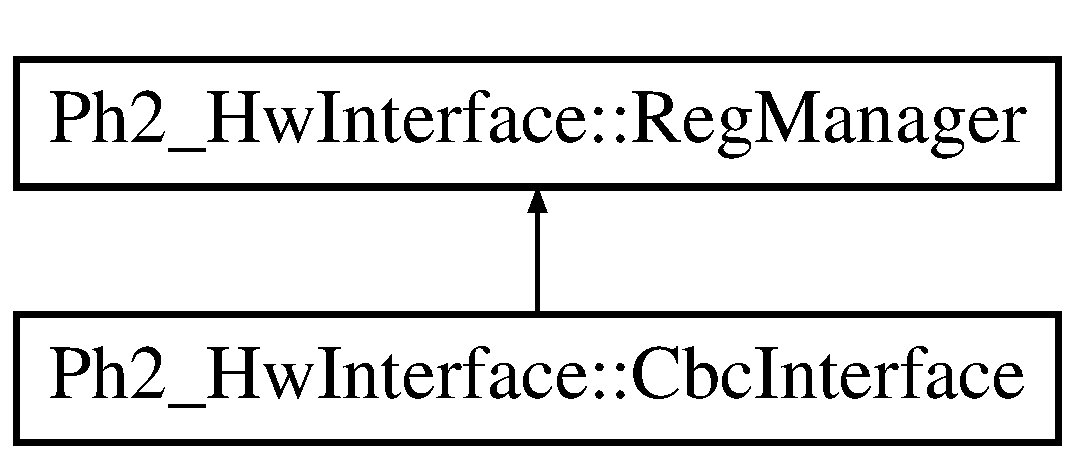
\includegraphics[height=2.000000cm]{class_ph2___hw_interface_1_1_cbc_interface}
\end{center}
\end{figure}
\subsection*{Public Member Functions}
\begin{DoxyCompactItemize}
\item 
\hypertarget{class_ph2___hw_interface_1_1_cbc_interface_a3ddefe5549da06a7d26fee1502a792b4}{{\bfseries Cbc\-Interface} (const char $\ast$pu\-Hal\-Config\-File\-Name)}\label{class_ph2___hw_interface_1_1_cbc_interface_a3ddefe5549da06a7d26fee1502a792b4}

\item 
\hypertarget{class_ph2___hw_interface_1_1_cbc_interface_af5cf4eb5b7134835f00349cb19f35c56}{void \hyperlink{class_ph2___hw_interface_1_1_cbc_interface_af5cf4eb5b7134835f00349cb19f35c56}{Configure\-Cbc} (Cbc \&p\-Cbc)}\label{class_ph2___hw_interface_1_1_cbc_interface_af5cf4eb5b7134835f00349cb19f35c56}

\begin{DoxyCompactList}\small\item\em Configure the Cbc after the Cbc\-Config\-File. \end{DoxyCompactList}\item 
\hypertarget{class_ph2___hw_interface_1_1_cbc_interface_a498d71b5709e0524b8e9dc50b92d1424}{void \hyperlink{class_ph2___hw_interface_1_1_cbc_interface_a498d71b5709e0524b8e9dc50b92d1424}{Update\-Cbc\-Write} (Cbc \&p\-Cbc, const std\-::string \&p\-Reg\-Node, uint32\-\_\-t \&p\-Word)}\label{class_ph2___hw_interface_1_1_cbc_interface_a498d71b5709e0524b8e9dc50b92d1424}

\begin{DoxyCompactList}\small\item\em Write the designated register in both Cbc and Cbc\-Config\-File. \end{DoxyCompactList}\item 
\hypertarget{class_ph2___hw_interface_1_1_cbc_interface_ab08ea1de98fe120098a4f5c52e017393}{void \hyperlink{class_ph2___hw_interface_1_1_cbc_interface_ab08ea1de98fe120098a4f5c52e017393}{Update\-Cbc\-Read} (Cbc \&p\-Cbc, const std\-::string \&p\-Reg\-Node)}\label{class_ph2___hw_interface_1_1_cbc_interface_ab08ea1de98fe120098a4f5c52e017393}

\begin{DoxyCompactList}\small\item\em Read the designated register in the Cbc and update the Cbc\-Config\-File. \end{DoxyCompactList}\end{DoxyCompactItemize}
\subsection*{Static Public Attributes}
\begin{DoxyCompactItemize}
\item 
\hypertarget{class_ph2___hw_interface_1_1_cbc_interface_ab45dcb5563c94075ac0a3e17d17c1fd4}{static const std\-::string {\bfseries f\-Str\-I2c\-Settings} = I2\-C\-\_\-\-S\-E\-T\-T\-I\-N\-G\-S}\label{class_ph2___hw_interface_1_1_cbc_interface_ab45dcb5563c94075ac0a3e17d17c1fd4}

\item 
\hypertarget{class_ph2___hw_interface_1_1_cbc_interface_a350e32baca2a50220eeff24b9fa07054}{static const std\-::string {\bfseries f\-Str\-I2c\-Command} = I2\-C\-\_\-\-C\-O\-M\-M\-A\-N\-D}\label{class_ph2___hw_interface_1_1_cbc_interface_a350e32baca2a50220eeff24b9fa07054}

\item 
\hypertarget{class_ph2___hw_interface_1_1_cbc_interface_a6a0730099e121a7707615ba6969afe80}{static const std\-::string {\bfseries f\-Str\-I2c\-Reply} = I2\-C\-\_\-\-R\-E\-P\-L\-Y}\label{class_ph2___hw_interface_1_1_cbc_interface_a6a0730099e121a7707615ba6969afe80}

\item 
\hypertarget{class_ph2___hw_interface_1_1_cbc_interface_ad5257bb9fac0efe9cb8307a04f51ef77}{static const uint32\-\_\-t {\bfseries f\-I2c\-Slave} = I2\-C\-\_\-\-S\-L\-A\-V\-E}\label{class_ph2___hw_interface_1_1_cbc_interface_ad5257bb9fac0efe9cb8307a04f51ef77}

\end{DoxyCompactItemize}
\subsection*{Additional Inherited Members}


The documentation for this class was generated from the following files\-:\begin{DoxyCompactItemize}
\item 
Cbc\-Interface.\-h\item 
Cbc\-Interface.\-cc\end{DoxyCompactItemize}

\hypertarget{class_ph2___hw_interface_1_1_exception}{
\section{Ph2\_\-Hw\-Interface::Exception Class Reference}
\label{class_ph2___hw_interface_1_1_exception}\index{Ph2_HwInterface::Exception@{Ph2\_\-HwInterface::Exception}}
}
\hyperlink{class_ph2___hw_interface_1_1_exception}{Exception} handling class, inheriting from std::exception.  


{\tt \#include $<$Exception.h$>$}

\subsection*{Public Member Functions}
\begin{CompactItemize}
\item 
\hyperlink{class_ph2___hw_interface_1_1_exception_9ac7df51fe36dfb65ff24ca975ec846f}{Exception} (const char $\ast$p\-Str\-Error)
\begin{CompactList}\small\item\em Constructor of \hyperlink{class_ph2___hw_interface_1_1_exception}{Exception} class. \item\end{CompactList}\item 
\hyperlink{class_ph2___hw_interface_1_1_exception_667217cdbe920cb69842a3d3afb69d35}{$\sim$Exception} ()  throw ()
\begin{CompactList}\small\item\em Destructor of \hyperlink{class_ph2___hw_interface_1_1_exception}{Exception} class. \item\end{CompactList}\item 
const char $\ast$ \hyperlink{class_ph2___hw_interface_1_1_exception_8db77fef785111589956a21598b748e0}{what} () const   throw ()
\begin{CompactList}\small\item\em What to throw. \item\end{CompactList}\end{CompactItemize}
\subsection*{Private Attributes}
\begin{CompactItemize}
\item 
std::string \hyperlink{class_ph2___hw_interface_1_1_exception_a060af06e0614e117e2902f41e57e179}{f\-Str\-Error}
\end{CompactItemize}


\subsection{Detailed Description}
\hyperlink{class_ph2___hw_interface_1_1_exception}{Exception} handling class, inheriting from std::exception. 



\subsection{Constructor \& Destructor Documentation}
\hypertarget{class_ph2___hw_interface_1_1_exception_9ac7df51fe36dfb65ff24ca975ec846f}{
\index{Ph2_HwInterface::Exception@{Ph2\_\-Hw\-Interface::Exception}!Exception@{Exception}}
\index{Exception@{Exception}!Ph2_HwInterface::Exception@{Ph2\_\-Hw\-Interface::Exception}}
\subsubsection[Exception]{\setlength{\rightskip}{0pt plus 5cm}Ph2\_\-Hw\-Interface::Exception::Exception (const char $\ast$ {\em p\-Str\-Error})\hspace{0.3cm}{\tt  \mbox{[}inline\mbox{]}}}}
\label{class_ph2___hw_interface_1_1_exception_9ac7df51fe36dfb65ff24ca975ec846f}


Constructor of \hyperlink{class_ph2___hw_interface_1_1_exception}{Exception} class. 

\begin{Desc}
\item[Parameters:]
\begin{description}
\item[{\em p\-Str\-Error}]: Error message \end{description}
\end{Desc}
\hypertarget{class_ph2___hw_interface_1_1_exception_667217cdbe920cb69842a3d3afb69d35}{
\index{Ph2_HwInterface::Exception@{Ph2\_\-Hw\-Interface::Exception}!~Exception@{$\sim$Exception}}
\index{~Exception@{$\sim$Exception}!Ph2_HwInterface::Exception@{Ph2\_\-Hw\-Interface::Exception}}
\subsubsection[$\sim$Exception]{\setlength{\rightskip}{0pt plus 5cm}Ph2\_\-Hw\-Interface::Exception::$\sim$Exception ()  throw ()\hspace{0.3cm}{\tt  \mbox{[}inline\mbox{]}}}}
\label{class_ph2___hw_interface_1_1_exception_667217cdbe920cb69842a3d3afb69d35}


Destructor of \hyperlink{class_ph2___hw_interface_1_1_exception}{Exception} class. 



\subsection{Member Function Documentation}
\hypertarget{class_ph2___hw_interface_1_1_exception_8db77fef785111589956a21598b748e0}{
\index{Ph2_HwInterface::Exception@{Ph2\_\-Hw\-Interface::Exception}!what@{what}}
\index{what@{what}!Ph2_HwInterface::Exception@{Ph2\_\-Hw\-Interface::Exception}}
\subsubsection[what]{\setlength{\rightskip}{0pt plus 5cm}const char $\ast$ Ph2\_\-Hw\-Interface::Exception::what () const  throw ()}}
\label{class_ph2___hw_interface_1_1_exception_8db77fef785111589956a21598b748e0}


What to throw. 



\subsection{Field Documentation}
\hypertarget{class_ph2___hw_interface_1_1_exception_a060af06e0614e117e2902f41e57e179}{
\index{Ph2_HwInterface::Exception@{Ph2\_\-Hw\-Interface::Exception}!fStrError@{fStrError}}
\index{fStrError@{fStrError}!Ph2_HwInterface::Exception@{Ph2\_\-Hw\-Interface::Exception}}
\subsubsection[fStrError]{\setlength{\rightskip}{0pt plus 5cm}std::string \hyperlink{class_ph2___hw_interface_1_1_exception_a060af06e0614e117e2902f41e57e179}{Ph2\_\-Hw\-Interface::Exception::f\-Str\-Error}\hspace{0.3cm}{\tt  \mbox{[}private\mbox{]}}}}
\label{class_ph2___hw_interface_1_1_exception_a060af06e0614e117e2902f41e57e179}


Error String 

The documentation for this class was generated from the following files:\begin{CompactItemize}
\item 
Utils/\hyperlink{_exception_8h}{Exception.h}\item 
Utils/\hyperlink{_exception_8cc}{Exception.cc}\end{CompactItemize}

\hypertarget{class_ph2___hw_interface_1_1_glib_interface}{\section{Ph2\-\_\-\-Hw\-Interface\-:\-:Glib\-Interface Class Reference}
\label{class_ph2___hw_interface_1_1_glib_interface}\index{Ph2\-\_\-\-Hw\-Interface\-::\-Glib\-Interface@{Ph2\-\_\-\-Hw\-Interface\-::\-Glib\-Interface}}
}


Permit r/w given registers in the Glib you specify.  




{\ttfamily \#include $<$G\-L\-I\-B\-Interface.\-h$>$}

Inheritance diagram for Ph2\-\_\-\-Hw\-Interface\-:\-:Glib\-Interface\-:\begin{figure}[H]
\begin{center}
\leavevmode
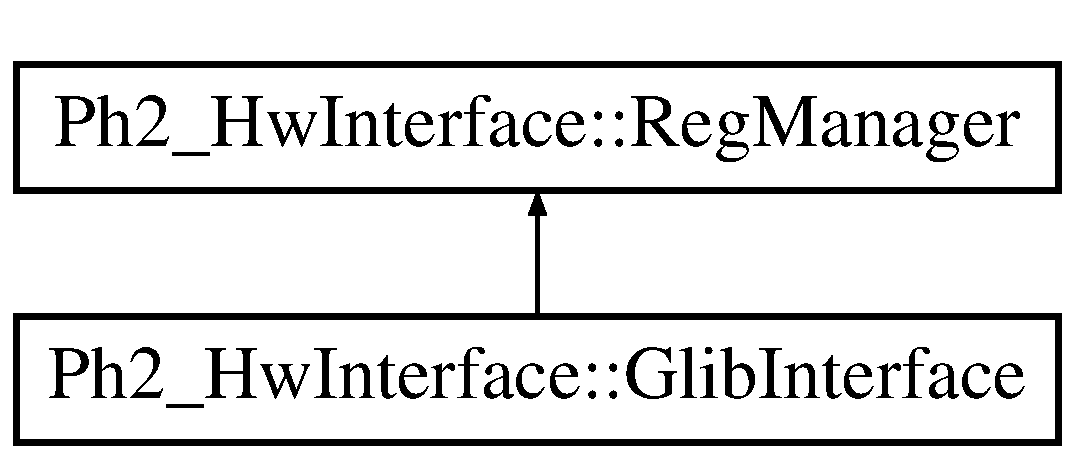
\includegraphics[height=2.000000cm]{class_ph2___hw_interface_1_1_glib_interface}
\end{center}
\end{figure}
\subsection*{Public Member Functions}
\begin{DoxyCompactItemize}
\item 
\hyperlink{class_ph2___hw_interface_1_1_glib_interface_a4aebde48748debad7e261c654c2c6fd8}{Glib\-Interface} (const char $\ast$pu\-Hal\-Config\-File\-Name)
\begin{DoxyCompactList}\small\item\em Constructor of the \hyperlink{class_ph2___hw_interface_1_1_glib_interface}{Glib\-Interface} class. \end{DoxyCompactList}\item 
\hyperlink{class_ph2___hw_interface_1_1_glib_interface_a1182c81cb29bca33b23a2c9f662df2ed}{$\sim$\-Glib\-Interface} ()
\begin{DoxyCompactList}\small\item\em Destructor of the \hyperlink{class_ph2___hw_interface_1_1_glib_interface}{Glib\-Interface} class. \end{DoxyCompactList}\item 
void \hyperlink{class_ph2___hw_interface_1_1_glib_interface_a51dd2e5a8128fd01a41c4d6b204df948}{get\-Board\-Info} (\hyperlink{class_ph2___hw_description_1_1_glib}{Glib} \&p\-Glib)
\begin{DoxyCompactList}\small\item\em Get the board infos. \end{DoxyCompactList}\item 
void \hyperlink{class_ph2___hw_interface_1_1_glib_interface_ad53d40d7cfea163bd3dcd04e233a02e3}{Select\-F\-E\-Id} (\hyperlink{class_ph2___hw_description_1_1_glib}{Glib} \&p\-Glib)
\begin{DoxyCompactList}\small\item\em Detect the right F\-E Id to write the right registers. \end{DoxyCompactList}\item 
void \hyperlink{class_ph2___hw_interface_1_1_glib_interface_aad68569190ea9b318b5be1abae4fd23f}{Configure\-Glib} (\hyperlink{class_ph2___hw_description_1_1_glib}{Glib} \&p\-Glib)
\begin{DoxyCompactList}\small\item\em Configure the Glib with its Config File. \end{DoxyCompactList}\item 
void \hyperlink{class_ph2___hw_interface_1_1_glib_interface_a0706eb396293fe5c8c717c5d0ab82165}{Start} (\hyperlink{class_ph2___hw_description_1_1_glib}{Glib} \&p\-Glib)
\begin{DoxyCompactList}\small\item\em Start a D\-A\-Q. \end{DoxyCompactList}\item 
void \hyperlink{class_ph2___hw_interface_1_1_glib_interface_a3073d292371ab4e602900f4276a43b6c}{Stop} (\hyperlink{class_ph2___hw_description_1_1_glib}{Glib} \&p\-Glib, uint32\-\_\-t p\-Nth\-Acq)
\begin{DoxyCompactList}\small\item\em Stop a D\-A\-Q. \end{DoxyCompactList}\item 
void \hyperlink{class_ph2___hw_interface_1_1_glib_interface_a1db7815b60c3e3637b23bfa27bab9692}{Pause} (\hyperlink{class_ph2___hw_description_1_1_glib}{Glib} \&p\-Glib)
\begin{DoxyCompactList}\small\item\em Pause a D\-A\-Q. \end{DoxyCompactList}\item 
void \hyperlink{class_ph2___hw_interface_1_1_glib_interface_a4d6568c22d8e3777ee909db37b3b01d6}{Unpause} (\hyperlink{class_ph2___hw_description_1_1_glib}{Glib} \&p\-Glib)
\begin{DoxyCompactList}\small\item\em Unpause a D\-A\-Q. \end{DoxyCompactList}\item 
void \hyperlink{class_ph2___hw_interface_1_1_glib_interface_ad3f91f03b0214987f4a9e8b63ff99dca}{Read\-Data} (\hyperlink{class_ph2___hw_description_1_1_glib}{Glib} \&p\-Glib, uint32\-\_\-t p\-Nth\-Acq, bool p\-Break\-Trigger)
\begin{DoxyCompactList}\small\item\em Read data from D\-A\-Q. \end{DoxyCompactList}\item 
void \hyperlink{class_ph2___hw_interface_1_1_glib_interface_a116aca1863dda40c52ca63259cd073b9}{Run} (\hyperlink{class_ph2___hw_description_1_1_glib}{Glib} \&p\-Glib)
\begin{DoxyCompactList}\small\item\em Run a D\-A\-Q. \end{DoxyCompactList}\item 
void \hyperlink{class_ph2___hw_interface_1_1_glib_interface_afeda624fe12657712e9f10cd60603d8a}{Update\-Glib\-Write} (\hyperlink{class_ph2___hw_description_1_1_glib}{Glib} \&p\-Glib, const std\-::string \&p\-Reg\-Node, const uint32\-\_\-t \&p\-Val)
\begin{DoxyCompactList}\small\item\em Update both Glib register and Config File. \end{DoxyCompactList}\item 
void \hyperlink{class_ph2___hw_interface_1_1_glib_interface_a1ab42500cf3f6369a8eb2404ef8cd85b}{Update\-Glib\-Read} (\hyperlink{class_ph2___hw_description_1_1_glib}{Glib} \&p\-Glib, const std\-::string \&p\-Reg\-Node)
\begin{DoxyCompactList}\small\item\em Update Config File with the value in the Glib register. \end{DoxyCompactList}\end{DoxyCompactItemize}
\subsection*{Data Fields}
\begin{DoxyCompactItemize}
\item 
\hyperlink{class_ph2___hw_interface_1_1_data}{Data} $\ast$ \hyperlink{class_ph2___hw_interface_1_1_glib_interface_ae0e95a15055342afd67e1f46aab1481c}{f\-Data}
\end{DoxyCompactItemize}
\subsection*{Private Member Functions}
\begin{DoxyCompactItemize}
\item 
void \hyperlink{class_ph2___hw_interface_1_1_glib_interface_a014fc0ea74353469aa54e4eecaffb225}{Select\-S\-R\-A\-M} (uint32\-\_\-t p\-Nth\-Acq)
\begin{DoxyCompactList}\small\item\em S\-R\-A\-M selection for D\-A\-Q. \end{DoxyCompactList}\end{DoxyCompactItemize}
\subsection*{Private Attributes}
\begin{DoxyCompactItemize}
\item 
unsigned int \hyperlink{class_ph2___hw_interface_1_1_glib_interface_a1b8fe11933c22b5c97e23ad2c4e4407c}{f\-N\-Total\-Acq}
\item 
bool \hyperlink{class_ph2___hw_interface_1_1_glib_interface_a0cc29dcdff019e8b11ea8ebab631159e}{f\-Stop}
\item 
struct timeval \hyperlink{class_ph2___hw_interface_1_1_glib_interface_a056c3192477cbd07c67ff822bc7123de}{f\-Start\-Veto}
\item 
std\-::string \hyperlink{class_ph2___hw_interface_1_1_glib_interface_a9e24a95e6ba16076ef8fbea1c96243f4}{f\-Str\-Sram}
\item 
std\-::string \hyperlink{class_ph2___hw_interface_1_1_glib_interface_a27b44db1be7f8a3802ba1a5d675a9888}{f\-Str\-Sram\-User\-Logic}
\item 
std\-::string \hyperlink{class_ph2___hw_interface_1_1_glib_interface_a40299b584632b402f3c54fc9d98d87f2}{f\-Str\-Full}
\item 
std\-::string \hyperlink{class_ph2___hw_interface_1_1_glib_interface_a925d65d022d0dc6d453e0e611826c377}{f\-Str\-Readout}
\item 
std\-::ofstream $\ast$ \hyperlink{class_ph2___hw_interface_1_1_glib_interface_a6efc2da55aafca870e1259e78436e1ef}{f\-Data\-File}
\end{DoxyCompactItemize}
\subsection*{Additional Inherited Members}


\subsection{Detailed Description}
Permit r/w given registers in the Glib you specify. 

\subsection{Constructor \& Destructor Documentation}
\hypertarget{class_ph2___hw_interface_1_1_glib_interface_a4aebde48748debad7e261c654c2c6fd8}{\index{Ph2\-\_\-\-Hw\-Interface\-::\-Glib\-Interface@{Ph2\-\_\-\-Hw\-Interface\-::\-Glib\-Interface}!Glib\-Interface@{Glib\-Interface}}
\index{Glib\-Interface@{Glib\-Interface}!Ph2_HwInterface::GlibInterface@{Ph2\-\_\-\-Hw\-Interface\-::\-Glib\-Interface}}
\subsubsection[{Glib\-Interface}]{\setlength{\rightskip}{0pt plus 5cm}Ph2\-\_\-\-Hw\-Interface\-::\-Glib\-Interface\-::\-Glib\-Interface (
\begin{DoxyParamCaption}
\item[{const char $\ast$}]{pu\-Hal\-Config\-File\-Name}
\end{DoxyParamCaption}
)}}\label{class_ph2___hw_interface_1_1_glib_interface_a4aebde48748debad7e261c654c2c6fd8}


Constructor of the \hyperlink{class_ph2___hw_interface_1_1_glib_interface}{Glib\-Interface} class. 


\begin{DoxyParams}{Parameters}
{\em pu\-Hal\-Config\-File\-Name} & \-: path of the u\-Hal Config File \\
\hline
\end{DoxyParams}
\hypertarget{class_ph2___hw_interface_1_1_glib_interface_a1182c81cb29bca33b23a2c9f662df2ed}{\index{Ph2\-\_\-\-Hw\-Interface\-::\-Glib\-Interface@{Ph2\-\_\-\-Hw\-Interface\-::\-Glib\-Interface}!$\sim$\-Glib\-Interface@{$\sim$\-Glib\-Interface}}
\index{$\sim$\-Glib\-Interface@{$\sim$\-Glib\-Interface}!Ph2_HwInterface::GlibInterface@{Ph2\-\_\-\-Hw\-Interface\-::\-Glib\-Interface}}
\subsubsection[{$\sim$\-Glib\-Interface}]{\setlength{\rightskip}{0pt plus 5cm}Ph2\-\_\-\-Hw\-Interface\-::\-Glib\-Interface\-::$\sim$\-Glib\-Interface (
\begin{DoxyParamCaption}
{}
\end{DoxyParamCaption}
)}}\label{class_ph2___hw_interface_1_1_glib_interface_a1182c81cb29bca33b23a2c9f662df2ed}


Destructor of the \hyperlink{class_ph2___hw_interface_1_1_glib_interface}{Glib\-Interface} class. 



\subsection{Member Function Documentation}
\hypertarget{class_ph2___hw_interface_1_1_glib_interface_aad68569190ea9b318b5be1abae4fd23f}{\index{Ph2\-\_\-\-Hw\-Interface\-::\-Glib\-Interface@{Ph2\-\_\-\-Hw\-Interface\-::\-Glib\-Interface}!Configure\-Glib@{Configure\-Glib}}
\index{Configure\-Glib@{Configure\-Glib}!Ph2_HwInterface::GlibInterface@{Ph2\-\_\-\-Hw\-Interface\-::\-Glib\-Interface}}
\subsubsection[{Configure\-Glib}]{\setlength{\rightskip}{0pt plus 5cm}void Ph2\-\_\-\-Hw\-Interface\-::\-Glib\-Interface\-::\-Configure\-Glib (
\begin{DoxyParamCaption}
\item[{{\bf Glib} \&}]{p\-Glib}
\end{DoxyParamCaption}
)}}\label{class_ph2___hw_interface_1_1_glib_interface_aad68569190ea9b318b5be1abae4fd23f}


Configure the Glib with its Config File. 


\begin{DoxyParams}{Parameters}
{\em p\-Glib} & \\
\hline
\end{DoxyParams}
\hypertarget{class_ph2___hw_interface_1_1_glib_interface_a51dd2e5a8128fd01a41c4d6b204df948}{\index{Ph2\-\_\-\-Hw\-Interface\-::\-Glib\-Interface@{Ph2\-\_\-\-Hw\-Interface\-::\-Glib\-Interface}!get\-Board\-Info@{get\-Board\-Info}}
\index{get\-Board\-Info@{get\-Board\-Info}!Ph2_HwInterface::GlibInterface@{Ph2\-\_\-\-Hw\-Interface\-::\-Glib\-Interface}}
\subsubsection[{get\-Board\-Info}]{\setlength{\rightskip}{0pt plus 5cm}void Ph2\-\_\-\-Hw\-Interface\-::\-Glib\-Interface\-::get\-Board\-Info (
\begin{DoxyParamCaption}
\item[{{\bf Glib} \&}]{p\-Glib}
\end{DoxyParamCaption}
)}}\label{class_ph2___hw_interface_1_1_glib_interface_a51dd2e5a8128fd01a41c4d6b204df948}


Get the board infos. 


\begin{DoxyParams}{Parameters}
{\em p\-Glib} & \\
\hline
\end{DoxyParams}
\hypertarget{class_ph2___hw_interface_1_1_glib_interface_a1db7815b60c3e3637b23bfa27bab9692}{\index{Ph2\-\_\-\-Hw\-Interface\-::\-Glib\-Interface@{Ph2\-\_\-\-Hw\-Interface\-::\-Glib\-Interface}!Pause@{Pause}}
\index{Pause@{Pause}!Ph2_HwInterface::GlibInterface@{Ph2\-\_\-\-Hw\-Interface\-::\-Glib\-Interface}}
\subsubsection[{Pause}]{\setlength{\rightskip}{0pt plus 5cm}void Ph2\-\_\-\-Hw\-Interface\-::\-Glib\-Interface\-::\-Pause (
\begin{DoxyParamCaption}
\item[{{\bf Glib} \&}]{p\-Glib}
\end{DoxyParamCaption}
)}}\label{class_ph2___hw_interface_1_1_glib_interface_a1db7815b60c3e3637b23bfa27bab9692}


Pause a D\-A\-Q. 


\begin{DoxyParams}{Parameters}
{\em p\-Glib} & \\
\hline
\end{DoxyParams}
\hypertarget{class_ph2___hw_interface_1_1_glib_interface_ad3f91f03b0214987f4a9e8b63ff99dca}{\index{Ph2\-\_\-\-Hw\-Interface\-::\-Glib\-Interface@{Ph2\-\_\-\-Hw\-Interface\-::\-Glib\-Interface}!Read\-Data@{Read\-Data}}
\index{Read\-Data@{Read\-Data}!Ph2_HwInterface::GlibInterface@{Ph2\-\_\-\-Hw\-Interface\-::\-Glib\-Interface}}
\subsubsection[{Read\-Data}]{\setlength{\rightskip}{0pt plus 5cm}void Ph2\-\_\-\-Hw\-Interface\-::\-Glib\-Interface\-::\-Read\-Data (
\begin{DoxyParamCaption}
\item[{{\bf Glib} \&}]{p\-Glib, }
\item[{uint32\-\_\-t}]{p\-Nth\-Acq, }
\item[{bool}]{p\-Break\-Trigger}
\end{DoxyParamCaption}
)}}\label{class_ph2___hw_interface_1_1_glib_interface_ad3f91f03b0214987f4a9e8b63ff99dca}


Read data from D\-A\-Q. 


\begin{DoxyParams}{Parameters}
{\em p\-Glib} & \\
\hline
{\em p\-Nth\-Acq} & \-: actual number of acquisitions \\
\hline
{\em p\-Break\-Trigger} & \-: if true, enable the break trigger \\
\hline
\end{DoxyParams}
\hypertarget{class_ph2___hw_interface_1_1_glib_interface_a116aca1863dda40c52ca63259cd073b9}{\index{Ph2\-\_\-\-Hw\-Interface\-::\-Glib\-Interface@{Ph2\-\_\-\-Hw\-Interface\-::\-Glib\-Interface}!Run@{Run}}
\index{Run@{Run}!Ph2_HwInterface::GlibInterface@{Ph2\-\_\-\-Hw\-Interface\-::\-Glib\-Interface}}
\subsubsection[{Run}]{\setlength{\rightskip}{0pt plus 5cm}void Ph2\-\_\-\-Hw\-Interface\-::\-Glib\-Interface\-::\-Run (
\begin{DoxyParamCaption}
\item[{{\bf Glib} \&}]{p\-Glib}
\end{DoxyParamCaption}
)}}\label{class_ph2___hw_interface_1_1_glib_interface_a116aca1863dda40c52ca63259cd073b9}


Run a D\-A\-Q. 


\begin{DoxyParams}{Parameters}
{\em p\-Glib} & \\
\hline
\end{DoxyParams}
\hypertarget{class_ph2___hw_interface_1_1_glib_interface_ad53d40d7cfea163bd3dcd04e233a02e3}{\index{Ph2\-\_\-\-Hw\-Interface\-::\-Glib\-Interface@{Ph2\-\_\-\-Hw\-Interface\-::\-Glib\-Interface}!Select\-F\-E\-Id@{Select\-F\-E\-Id}}
\index{Select\-F\-E\-Id@{Select\-F\-E\-Id}!Ph2_HwInterface::GlibInterface@{Ph2\-\_\-\-Hw\-Interface\-::\-Glib\-Interface}}
\subsubsection[{Select\-F\-E\-Id}]{\setlength{\rightskip}{0pt plus 5cm}void Ph2\-\_\-\-Hw\-Interface\-::\-Glib\-Interface\-::\-Select\-F\-E\-Id (
\begin{DoxyParamCaption}
\item[{{\bf Glib} \&}]{p\-Glib}
\end{DoxyParamCaption}
)}}\label{class_ph2___hw_interface_1_1_glib_interface_ad53d40d7cfea163bd3dcd04e233a02e3}


Detect the right F\-E Id to write the right registers. 


\begin{DoxyParams}{Parameters}
{\em p\-Glib} & \\
\hline
\end{DoxyParams}
\hypertarget{class_ph2___hw_interface_1_1_glib_interface_a014fc0ea74353469aa54e4eecaffb225}{\index{Ph2\-\_\-\-Hw\-Interface\-::\-Glib\-Interface@{Ph2\-\_\-\-Hw\-Interface\-::\-Glib\-Interface}!Select\-S\-R\-A\-M@{Select\-S\-R\-A\-M}}
\index{Select\-S\-R\-A\-M@{Select\-S\-R\-A\-M}!Ph2_HwInterface::GlibInterface@{Ph2\-\_\-\-Hw\-Interface\-::\-Glib\-Interface}}
\subsubsection[{Select\-S\-R\-A\-M}]{\setlength{\rightskip}{0pt plus 5cm}void Ph2\-\_\-\-Hw\-Interface\-::\-Glib\-Interface\-::\-Select\-S\-R\-A\-M (
\begin{DoxyParamCaption}
\item[{uint32\-\_\-t}]{p\-Nth\-Acq}
\end{DoxyParamCaption}
)\hspace{0.3cm}{\ttfamily [private]}}}\label{class_ph2___hw_interface_1_1_glib_interface_a014fc0ea74353469aa54e4eecaffb225}


S\-R\-A\-M selection for D\-A\-Q. 


\begin{DoxyParams}{Parameters}
{\em p\-Nth\-Acq} & \-: actual number of acquisitions \\
\hline
\end{DoxyParams}
\hypertarget{class_ph2___hw_interface_1_1_glib_interface_a0706eb396293fe5c8c717c5d0ab82165}{\index{Ph2\-\_\-\-Hw\-Interface\-::\-Glib\-Interface@{Ph2\-\_\-\-Hw\-Interface\-::\-Glib\-Interface}!Start@{Start}}
\index{Start@{Start}!Ph2_HwInterface::GlibInterface@{Ph2\-\_\-\-Hw\-Interface\-::\-Glib\-Interface}}
\subsubsection[{Start}]{\setlength{\rightskip}{0pt plus 5cm}void Ph2\-\_\-\-Hw\-Interface\-::\-Glib\-Interface\-::\-Start (
\begin{DoxyParamCaption}
\item[{{\bf Glib} \&}]{p\-Glib}
\end{DoxyParamCaption}
)}}\label{class_ph2___hw_interface_1_1_glib_interface_a0706eb396293fe5c8c717c5d0ab82165}


Start a D\-A\-Q. 


\begin{DoxyParams}{Parameters}
{\em p\-Glib} & \\
\hline
\end{DoxyParams}
\hypertarget{class_ph2___hw_interface_1_1_glib_interface_a3073d292371ab4e602900f4276a43b6c}{\index{Ph2\-\_\-\-Hw\-Interface\-::\-Glib\-Interface@{Ph2\-\_\-\-Hw\-Interface\-::\-Glib\-Interface}!Stop@{Stop}}
\index{Stop@{Stop}!Ph2_HwInterface::GlibInterface@{Ph2\-\_\-\-Hw\-Interface\-::\-Glib\-Interface}}
\subsubsection[{Stop}]{\setlength{\rightskip}{0pt plus 5cm}void Ph2\-\_\-\-Hw\-Interface\-::\-Glib\-Interface\-::\-Stop (
\begin{DoxyParamCaption}
\item[{{\bf Glib} \&}]{p\-Glib, }
\item[{uint32\-\_\-t}]{p\-Nth\-Acq}
\end{DoxyParamCaption}
)}}\label{class_ph2___hw_interface_1_1_glib_interface_a3073d292371ab4e602900f4276a43b6c}


Stop a D\-A\-Q. 


\begin{DoxyParams}{Parameters}
{\em p\-Glib} & \\
\hline
{\em p\-Nth\-Acq} & \-: actual number of acquisitions \\
\hline
\end{DoxyParams}
\hypertarget{class_ph2___hw_interface_1_1_glib_interface_a4d6568c22d8e3777ee909db37b3b01d6}{\index{Ph2\-\_\-\-Hw\-Interface\-::\-Glib\-Interface@{Ph2\-\_\-\-Hw\-Interface\-::\-Glib\-Interface}!Unpause@{Unpause}}
\index{Unpause@{Unpause}!Ph2_HwInterface::GlibInterface@{Ph2\-\_\-\-Hw\-Interface\-::\-Glib\-Interface}}
\subsubsection[{Unpause}]{\setlength{\rightskip}{0pt plus 5cm}void Ph2\-\_\-\-Hw\-Interface\-::\-Glib\-Interface\-::\-Unpause (
\begin{DoxyParamCaption}
\item[{{\bf Glib} \&}]{p\-Glib}
\end{DoxyParamCaption}
)}}\label{class_ph2___hw_interface_1_1_glib_interface_a4d6568c22d8e3777ee909db37b3b01d6}


Unpause a D\-A\-Q. 


\begin{DoxyParams}{Parameters}
{\em p\-Glib} & \\
\hline
\end{DoxyParams}
\hypertarget{class_ph2___hw_interface_1_1_glib_interface_a1ab42500cf3f6369a8eb2404ef8cd85b}{\index{Ph2\-\_\-\-Hw\-Interface\-::\-Glib\-Interface@{Ph2\-\_\-\-Hw\-Interface\-::\-Glib\-Interface}!Update\-Glib\-Read@{Update\-Glib\-Read}}
\index{Update\-Glib\-Read@{Update\-Glib\-Read}!Ph2_HwInterface::GlibInterface@{Ph2\-\_\-\-Hw\-Interface\-::\-Glib\-Interface}}
\subsubsection[{Update\-Glib\-Read}]{\setlength{\rightskip}{0pt plus 5cm}void Ph2\-\_\-\-Hw\-Interface\-::\-Glib\-Interface\-::\-Update\-Glib\-Read (
\begin{DoxyParamCaption}
\item[{{\bf Glib} \&}]{p\-Glib, }
\item[{const std\-::string \&}]{p\-Reg\-Node}
\end{DoxyParamCaption}
)}}\label{class_ph2___hw_interface_1_1_glib_interface_a1ab42500cf3f6369a8eb2404ef8cd85b}


Update Config File with the value in the Glib register. 


\begin{DoxyParams}{Parameters}
{\em p\-Glib} & \\
\hline
{\em p\-Reg\-Node} & \-: Node of the register to update \\
\hline
\end{DoxyParams}
\hypertarget{class_ph2___hw_interface_1_1_glib_interface_afeda624fe12657712e9f10cd60603d8a}{\index{Ph2\-\_\-\-Hw\-Interface\-::\-Glib\-Interface@{Ph2\-\_\-\-Hw\-Interface\-::\-Glib\-Interface}!Update\-Glib\-Write@{Update\-Glib\-Write}}
\index{Update\-Glib\-Write@{Update\-Glib\-Write}!Ph2_HwInterface::GlibInterface@{Ph2\-\_\-\-Hw\-Interface\-::\-Glib\-Interface}}
\subsubsection[{Update\-Glib\-Write}]{\setlength{\rightskip}{0pt plus 5cm}void Ph2\-\_\-\-Hw\-Interface\-::\-Glib\-Interface\-::\-Update\-Glib\-Write (
\begin{DoxyParamCaption}
\item[{{\bf Glib} \&}]{p\-Glib, }
\item[{const std\-::string \&}]{p\-Reg\-Node, }
\item[{const uint32\-\_\-t \&}]{p\-Val}
\end{DoxyParamCaption}
)}}\label{class_ph2___hw_interface_1_1_glib_interface_afeda624fe12657712e9f10cd60603d8a}


Update both Glib register and Config File. 


\begin{DoxyParams}{Parameters}
{\em p\-Glib} & \\
\hline
{\em p\-Reg\-Node} & \-: Node of the register to update \\
\hline
{\em p\-Val} & \-: Value to write \\
\hline
\end{DoxyParams}


\subsection{Field Documentation}
\hypertarget{class_ph2___hw_interface_1_1_glib_interface_ae0e95a15055342afd67e1f46aab1481c}{\index{Ph2\-\_\-\-Hw\-Interface\-::\-Glib\-Interface@{Ph2\-\_\-\-Hw\-Interface\-::\-Glib\-Interface}!f\-Data@{f\-Data}}
\index{f\-Data@{f\-Data}!Ph2_HwInterface::GlibInterface@{Ph2\-\_\-\-Hw\-Interface\-::\-Glib\-Interface}}
\subsubsection[{f\-Data}]{\setlength{\rightskip}{0pt plus 5cm}{\bf Data}$\ast$ Ph2\-\_\-\-Hw\-Interface\-::\-Glib\-Interface\-::f\-Data}}\label{class_ph2___hw_interface_1_1_glib_interface_ae0e95a15055342afd67e1f46aab1481c}
\hyperlink{class_ph2___hw_interface_1_1_data}{Data} read storage \hypertarget{class_ph2___hw_interface_1_1_glib_interface_a6efc2da55aafca870e1259e78436e1ef}{\index{Ph2\-\_\-\-Hw\-Interface\-::\-Glib\-Interface@{Ph2\-\_\-\-Hw\-Interface\-::\-Glib\-Interface}!f\-Data\-File@{f\-Data\-File}}
\index{f\-Data\-File@{f\-Data\-File}!Ph2_HwInterface::GlibInterface@{Ph2\-\_\-\-Hw\-Interface\-::\-Glib\-Interface}}
\subsubsection[{f\-Data\-File}]{\setlength{\rightskip}{0pt plus 5cm}std\-::ofstream$\ast$ Ph2\-\_\-\-Hw\-Interface\-::\-Glib\-Interface\-::f\-Data\-File\hspace{0.3cm}{\ttfamily [private]}}}\label{class_ph2___hw_interface_1_1_glib_interface_a6efc2da55aafca870e1259e78436e1ef}
File storing data \hypertarget{class_ph2___hw_interface_1_1_glib_interface_a1b8fe11933c22b5c97e23ad2c4e4407c}{\index{Ph2\-\_\-\-Hw\-Interface\-::\-Glib\-Interface@{Ph2\-\_\-\-Hw\-Interface\-::\-Glib\-Interface}!f\-N\-Total\-Acq@{f\-N\-Total\-Acq}}
\index{f\-N\-Total\-Acq@{f\-N\-Total\-Acq}!Ph2_HwInterface::GlibInterface@{Ph2\-\_\-\-Hw\-Interface\-::\-Glib\-Interface}}
\subsubsection[{f\-N\-Total\-Acq}]{\setlength{\rightskip}{0pt plus 5cm}unsigned int Ph2\-\_\-\-Hw\-Interface\-::\-Glib\-Interface\-::f\-N\-Total\-Acq\hspace{0.3cm}{\ttfamily [private]}}}\label{class_ph2___hw_interface_1_1_glib_interface_a1b8fe11933c22b5c97e23ad2c4e4407c}
\hypertarget{class_ph2___hw_interface_1_1_glib_interface_a056c3192477cbd07c67ff822bc7123de}{\index{Ph2\-\_\-\-Hw\-Interface\-::\-Glib\-Interface@{Ph2\-\_\-\-Hw\-Interface\-::\-Glib\-Interface}!f\-Start\-Veto@{f\-Start\-Veto}}
\index{f\-Start\-Veto@{f\-Start\-Veto}!Ph2_HwInterface::GlibInterface@{Ph2\-\_\-\-Hw\-Interface\-::\-Glib\-Interface}}
\subsubsection[{f\-Start\-Veto}]{\setlength{\rightskip}{0pt plus 5cm}struct timeval Ph2\-\_\-\-Hw\-Interface\-::\-Glib\-Interface\-::f\-Start\-Veto\hspace{0.3cm}{\ttfamily [private]}}}\label{class_ph2___hw_interface_1_1_glib_interface_a056c3192477cbd07c67ff822bc7123de}
\hypertarget{class_ph2___hw_interface_1_1_glib_interface_a0cc29dcdff019e8b11ea8ebab631159e}{\index{Ph2\-\_\-\-Hw\-Interface\-::\-Glib\-Interface@{Ph2\-\_\-\-Hw\-Interface\-::\-Glib\-Interface}!f\-Stop@{f\-Stop}}
\index{f\-Stop@{f\-Stop}!Ph2_HwInterface::GlibInterface@{Ph2\-\_\-\-Hw\-Interface\-::\-Glib\-Interface}}
\subsubsection[{f\-Stop}]{\setlength{\rightskip}{0pt plus 5cm}bool Ph2\-\_\-\-Hw\-Interface\-::\-Glib\-Interface\-::f\-Stop\hspace{0.3cm}{\ttfamily [private]}}}\label{class_ph2___hw_interface_1_1_glib_interface_a0cc29dcdff019e8b11ea8ebab631159e}
\hypertarget{class_ph2___hw_interface_1_1_glib_interface_a40299b584632b402f3c54fc9d98d87f2}{\index{Ph2\-\_\-\-Hw\-Interface\-::\-Glib\-Interface@{Ph2\-\_\-\-Hw\-Interface\-::\-Glib\-Interface}!f\-Str\-Full@{f\-Str\-Full}}
\index{f\-Str\-Full@{f\-Str\-Full}!Ph2_HwInterface::GlibInterface@{Ph2\-\_\-\-Hw\-Interface\-::\-Glib\-Interface}}
\subsubsection[{f\-Str\-Full}]{\setlength{\rightskip}{0pt plus 5cm}std\-::string Ph2\-\_\-\-Hw\-Interface\-::\-Glib\-Interface\-::f\-Str\-Full\hspace{0.3cm}{\ttfamily [private]}}}\label{class_ph2___hw_interface_1_1_glib_interface_a40299b584632b402f3c54fc9d98d87f2}
\hypertarget{class_ph2___hw_interface_1_1_glib_interface_a925d65d022d0dc6d453e0e611826c377}{\index{Ph2\-\_\-\-Hw\-Interface\-::\-Glib\-Interface@{Ph2\-\_\-\-Hw\-Interface\-::\-Glib\-Interface}!f\-Str\-Readout@{f\-Str\-Readout}}
\index{f\-Str\-Readout@{f\-Str\-Readout}!Ph2_HwInterface::GlibInterface@{Ph2\-\_\-\-Hw\-Interface\-::\-Glib\-Interface}}
\subsubsection[{f\-Str\-Readout}]{\setlength{\rightskip}{0pt plus 5cm}std\-::string Ph2\-\_\-\-Hw\-Interface\-::\-Glib\-Interface\-::f\-Str\-Readout\hspace{0.3cm}{\ttfamily [private]}}}\label{class_ph2___hw_interface_1_1_glib_interface_a925d65d022d0dc6d453e0e611826c377}
\hypertarget{class_ph2___hw_interface_1_1_glib_interface_a9e24a95e6ba16076ef8fbea1c96243f4}{\index{Ph2\-\_\-\-Hw\-Interface\-::\-Glib\-Interface@{Ph2\-\_\-\-Hw\-Interface\-::\-Glib\-Interface}!f\-Str\-Sram@{f\-Str\-Sram}}
\index{f\-Str\-Sram@{f\-Str\-Sram}!Ph2_HwInterface::GlibInterface@{Ph2\-\_\-\-Hw\-Interface\-::\-Glib\-Interface}}
\subsubsection[{f\-Str\-Sram}]{\setlength{\rightskip}{0pt plus 5cm}std\-::string Ph2\-\_\-\-Hw\-Interface\-::\-Glib\-Interface\-::f\-Str\-Sram\hspace{0.3cm}{\ttfamily [private]}}}\label{class_ph2___hw_interface_1_1_glib_interface_a9e24a95e6ba16076ef8fbea1c96243f4}
\hypertarget{class_ph2___hw_interface_1_1_glib_interface_a27b44db1be7f8a3802ba1a5d675a9888}{\index{Ph2\-\_\-\-Hw\-Interface\-::\-Glib\-Interface@{Ph2\-\_\-\-Hw\-Interface\-::\-Glib\-Interface}!f\-Str\-Sram\-User\-Logic@{f\-Str\-Sram\-User\-Logic}}
\index{f\-Str\-Sram\-User\-Logic@{f\-Str\-Sram\-User\-Logic}!Ph2_HwInterface::GlibInterface@{Ph2\-\_\-\-Hw\-Interface\-::\-Glib\-Interface}}
\subsubsection[{f\-Str\-Sram\-User\-Logic}]{\setlength{\rightskip}{0pt plus 5cm}std\-::string Ph2\-\_\-\-Hw\-Interface\-::\-Glib\-Interface\-::f\-Str\-Sram\-User\-Logic\hspace{0.3cm}{\ttfamily [private]}}}\label{class_ph2___hw_interface_1_1_glib_interface_a27b44db1be7f8a3802ba1a5d675a9888}


The documentation for this class was generated from the following files\-:\begin{DoxyCompactItemize}
\item 
H\-W\-Interface/\hyperlink{_g_l_i_b_interface_8h}{G\-L\-I\-B\-Interface.\-h}\item 
H\-W\-Interface/\hyperlink{_g_l_i_b_interface_8cc}{G\-L\-I\-B\-Interface.\-cc}\end{DoxyCompactItemize}

\hypertarget{class_ph2___hw_interface_1_1_reg_manager}{\section{Ph2\-\_\-\-Hw\-Interface\-:\-:Reg\-Manager Class Reference}
\label{class_ph2___hw_interface_1_1_reg_manager}\index{Ph2\-\_\-\-Hw\-Interface\-::\-Reg\-Manager@{Ph2\-\_\-\-Hw\-Interface\-::\-Reg\-Manager}}
}


Permit connection to given boards and r/w given registers.  




{\ttfamily \#include $<$Reg\-Manager.\-h$>$}

Inheritance diagram for Ph2\-\_\-\-Hw\-Interface\-:\-:Reg\-Manager\-:\begin{figure}[H]
\begin{center}
\leavevmode
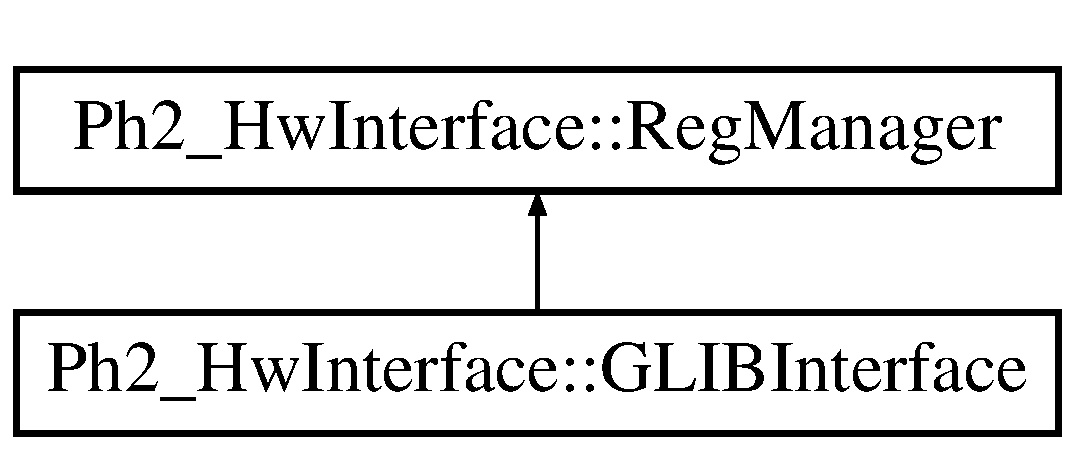
\includegraphics[height=2.000000cm]{class_ph2___hw_interface_1_1_reg_manager}
\end{center}
\end{figure}
\subsection*{Public Member Functions}
\begin{DoxyCompactItemize}
\item 
\hyperlink{class_ph2___hw_interface_1_1_reg_manager_a938f6b582b1fffcb478f35fd9d81954f}{Reg\-Manager} (const char $\ast$pu\-Hal\-Config\-File\-Name)
\begin{DoxyCompactList}\small\item\em Constructor of the \hyperlink{class_ph2___hw_interface_1_1_reg_manager}{Reg\-Manager} class. \end{DoxyCompactList}\item 
virtual \hyperlink{class_ph2___hw_interface_1_1_reg_manager_a5d650c4e6467153f98f999abbbfc354c}{$\sim$\-Reg\-Manager} ()
\begin{DoxyCompactList}\small\item\em Destructor of the \hyperlink{class_ph2___hw_interface_1_1_reg_manager}{Reg\-Manager} class. \end{DoxyCompactList}\end{DoxyCompactItemize}
\subsection*{Protected Member Functions}
\begin{DoxyCompactItemize}
\item 
virtual bool \hyperlink{class_ph2___hw_interface_1_1_reg_manager_a31174516fef6706c88c3f59dd93e4fdf}{Write\-Reg} (const std\-::string \&p\-Reg\-Node, const uint32\-\_\-t \&p\-Val)
\begin{DoxyCompactList}\small\item\em Write a register. \end{DoxyCompactList}\item 
virtual bool \hyperlink{class_ph2___hw_interface_1_1_reg_manager_a888f5cccb05daa28896cf622abfdcbd6}{Write\-Block\-Reg} (const std\-::string \&p\-Reg\-Node, const std\-::vector$<$ uint32\-\_\-t $>$ \&p\-Values)
\begin{DoxyCompactList}\small\item\em Write a block of values in a register. \end{DoxyCompactList}\item 
virtual uhal\-::\-Val\-Word$<$ uint32\-\_\-t $>$ \hyperlink{class_ph2___hw_interface_1_1_reg_manager_a077e0a18592206365150680213345112}{Read\-Reg} (const std\-::string \&p\-Reg\-Node)
\begin{DoxyCompactList}\small\item\em Read a value in a register. \end{DoxyCompactList}\item 
virtual uhal\-::\-Val\-Vector$<$ uint32\-\_\-t $>$ \hyperlink{class_ph2___hw_interface_1_1_reg_manager_a6481c211d27badc409ff0e7af20575e4}{Read\-Block\-Reg} (const std\-::string \&p\-Reg\-Node, const uint32\-\_\-t \&p\-Blocksize)
\begin{DoxyCompactList}\small\item\em Read a block of values in a register. \end{DoxyCompactList}\item 
virtual void \hyperlink{class_ph2___hw_interface_1_1_reg_manager_a20c502bcad5115c6ae16d4d356b72f0c}{Choose\-Board} (uint8\-\_\-t p\-Board\-Id)
\begin{DoxyCompactList}\small\item\em Choose the board we want to talk with. \end{DoxyCompactList}\end{DoxyCompactItemize}
\subsection*{Protected Attributes}
\begin{DoxyCompactItemize}
\item 
uhal\-::\-Hw\-Interface $\ast$ \hyperlink{class_ph2___hw_interface_1_1_reg_manager_a0d4908ec834a3a0b7d8139872fd0a4a0}{f\-Board}
\item 
const char $\ast$ \hyperlink{class_ph2___hw_interface_1_1_reg_manager_aaaa29ca65c283acc645132c7bef0f24f}{f\-U\-Hal\-Config\-File\-Name}
\item 
std\-::map$<$ uint8\-\_\-t, \\*
uhal\-::\-Hw\-Interface $\ast$ $>$ \hyperlink{class_ph2___hw_interface_1_1_reg_manager_a9c34ffe467a572796c05036533bb6d39}{f\-Board\-Map}
\end{DoxyCompactItemize}


\subsection{Detailed Description}
Permit connection to given boards and r/w given registers. 

\subsection{Constructor \& Destructor Documentation}
\hypertarget{class_ph2___hw_interface_1_1_reg_manager_a938f6b582b1fffcb478f35fd9d81954f}{\index{Ph2\-\_\-\-Hw\-Interface\-::\-Reg\-Manager@{Ph2\-\_\-\-Hw\-Interface\-::\-Reg\-Manager}!Reg\-Manager@{Reg\-Manager}}
\index{Reg\-Manager@{Reg\-Manager}!Ph2_HwInterface::RegManager@{Ph2\-\_\-\-Hw\-Interface\-::\-Reg\-Manager}}
\subsubsection[{Reg\-Manager}]{\setlength{\rightskip}{0pt plus 5cm}Ph2\-\_\-\-Hw\-Interface\-::\-Reg\-Manager\-::\-Reg\-Manager (
\begin{DoxyParamCaption}
\item[{const char $\ast$}]{pu\-Hal\-Config\-File\-Name}
\end{DoxyParamCaption}
)}}\label{class_ph2___hw_interface_1_1_reg_manager_a938f6b582b1fffcb478f35fd9d81954f}


Constructor of the \hyperlink{class_ph2___hw_interface_1_1_reg_manager}{Reg\-Manager} class. 


\begin{DoxyParams}{Parameters}
{\em pu\-Hal\-Config\-File\-Name} & \-: path of the u\-Hal Config File \\
\hline
\end{DoxyParams}
\hypertarget{class_ph2___hw_interface_1_1_reg_manager_a5d650c4e6467153f98f999abbbfc354c}{\index{Ph2\-\_\-\-Hw\-Interface\-::\-Reg\-Manager@{Ph2\-\_\-\-Hw\-Interface\-::\-Reg\-Manager}!$\sim$\-Reg\-Manager@{$\sim$\-Reg\-Manager}}
\index{$\sim$\-Reg\-Manager@{$\sim$\-Reg\-Manager}!Ph2_HwInterface::RegManager@{Ph2\-\_\-\-Hw\-Interface\-::\-Reg\-Manager}}
\subsubsection[{$\sim$\-Reg\-Manager}]{\setlength{\rightskip}{0pt plus 5cm}Ph2\-\_\-\-Hw\-Interface\-::\-Reg\-Manager\-::$\sim$\-Reg\-Manager (
\begin{DoxyParamCaption}
{}
\end{DoxyParamCaption}
)\hspace{0.3cm}{\ttfamily [virtual]}}}\label{class_ph2___hw_interface_1_1_reg_manager_a5d650c4e6467153f98f999abbbfc354c}


Destructor of the \hyperlink{class_ph2___hw_interface_1_1_reg_manager}{Reg\-Manager} class. 



\subsection{Member Function Documentation}
\hypertarget{class_ph2___hw_interface_1_1_reg_manager_a20c502bcad5115c6ae16d4d356b72f0c}{\index{Ph2\-\_\-\-Hw\-Interface\-::\-Reg\-Manager@{Ph2\-\_\-\-Hw\-Interface\-::\-Reg\-Manager}!Choose\-Board@{Choose\-Board}}
\index{Choose\-Board@{Choose\-Board}!Ph2_HwInterface::RegManager@{Ph2\-\_\-\-Hw\-Interface\-::\-Reg\-Manager}}
\subsubsection[{Choose\-Board}]{\setlength{\rightskip}{0pt plus 5cm}void Ph2\-\_\-\-Hw\-Interface\-::\-Reg\-Manager\-::\-Choose\-Board (
\begin{DoxyParamCaption}
\item[{uint8\-\_\-t}]{p\-Board\-Id}
\end{DoxyParamCaption}
)\hspace{0.3cm}{\ttfamily [protected]}, {\ttfamily [virtual]}}}\label{class_ph2___hw_interface_1_1_reg_manager_a20c502bcad5115c6ae16d4d356b72f0c}


Choose the board we want to talk with. 


\begin{DoxyParams}{Parameters}
{\em p\-Board\-Id} & \-: Id of the Board to connect to \\
\hline
\end{DoxyParams}
\hypertarget{class_ph2___hw_interface_1_1_reg_manager_a6481c211d27badc409ff0e7af20575e4}{\index{Ph2\-\_\-\-Hw\-Interface\-::\-Reg\-Manager@{Ph2\-\_\-\-Hw\-Interface\-::\-Reg\-Manager}!Read\-Block\-Reg@{Read\-Block\-Reg}}
\index{Read\-Block\-Reg@{Read\-Block\-Reg}!Ph2_HwInterface::RegManager@{Ph2\-\_\-\-Hw\-Interface\-::\-Reg\-Manager}}
\subsubsection[{Read\-Block\-Reg}]{\setlength{\rightskip}{0pt plus 5cm}uhal\-::\-Val\-Vector$<$ uint32\-\_\-t $>$ Ph2\-\_\-\-Hw\-Interface\-::\-Reg\-Manager\-::\-Read\-Block\-Reg (
\begin{DoxyParamCaption}
\item[{const std\-::string \&}]{p\-Reg\-Node, }
\item[{const uint32\-\_\-t \&}]{p\-Blocksize}
\end{DoxyParamCaption}
)\hspace{0.3cm}{\ttfamily [protected]}, {\ttfamily [virtual]}}}\label{class_ph2___hw_interface_1_1_reg_manager_a6481c211d27badc409ff0e7af20575e4}


Read a block of values in a register. 


\begin{DoxyParams}{Parameters}
{\em p\-Reg\-Node} & \-: Node of the register to read \\
\hline
{\em p\-Blocksize} & \-: Size of the block to read \\
\hline
\end{DoxyParams}
\begin{DoxyReturn}{Returns}
Val\-Vector block values of the register 
\end{DoxyReturn}
\hypertarget{class_ph2___hw_interface_1_1_reg_manager_a077e0a18592206365150680213345112}{\index{Ph2\-\_\-\-Hw\-Interface\-::\-Reg\-Manager@{Ph2\-\_\-\-Hw\-Interface\-::\-Reg\-Manager}!Read\-Reg@{Read\-Reg}}
\index{Read\-Reg@{Read\-Reg}!Ph2_HwInterface::RegManager@{Ph2\-\_\-\-Hw\-Interface\-::\-Reg\-Manager}}
\subsubsection[{Read\-Reg}]{\setlength{\rightskip}{0pt plus 5cm}uhal\-::\-Val\-Word$<$ uint32\-\_\-t $>$ Ph2\-\_\-\-Hw\-Interface\-::\-Reg\-Manager\-::\-Read\-Reg (
\begin{DoxyParamCaption}
\item[{const std\-::string \&}]{p\-Reg\-Node}
\end{DoxyParamCaption}
)\hspace{0.3cm}{\ttfamily [protected]}, {\ttfamily [virtual]}}}\label{class_ph2___hw_interface_1_1_reg_manager_a077e0a18592206365150680213345112}


Read a value in a register. 


\begin{DoxyParams}{Parameters}
{\em p\-Reg\-Node} & \-: Node of the register to read \\
\hline
\end{DoxyParams}
\begin{DoxyReturn}{Returns}
Val\-Word value of the register 
\end{DoxyReturn}
\hypertarget{class_ph2___hw_interface_1_1_reg_manager_a888f5cccb05daa28896cf622abfdcbd6}{\index{Ph2\-\_\-\-Hw\-Interface\-::\-Reg\-Manager@{Ph2\-\_\-\-Hw\-Interface\-::\-Reg\-Manager}!Write\-Block\-Reg@{Write\-Block\-Reg}}
\index{Write\-Block\-Reg@{Write\-Block\-Reg}!Ph2_HwInterface::RegManager@{Ph2\-\_\-\-Hw\-Interface\-::\-Reg\-Manager}}
\subsubsection[{Write\-Block\-Reg}]{\setlength{\rightskip}{0pt plus 5cm}bool Ph2\-\_\-\-Hw\-Interface\-::\-Reg\-Manager\-::\-Write\-Block\-Reg (
\begin{DoxyParamCaption}
\item[{const std\-::string \&}]{p\-Reg\-Node, }
\item[{const std\-::vector$<$ uint32\-\_\-t $>$ \&}]{p\-Values}
\end{DoxyParamCaption}
)\hspace{0.3cm}{\ttfamily [protected]}, {\ttfamily [virtual]}}}\label{class_ph2___hw_interface_1_1_reg_manager_a888f5cccb05daa28896cf622abfdcbd6}


Write a block of values in a register. 


\begin{DoxyParams}{Parameters}
{\em p\-Reg\-Node} & \-: Node of the register to write \\
\hline
{\em p\-Values} & \-: Block of values to write \\
\hline
\end{DoxyParams}
\begin{DoxyReturn}{Returns}
boolean confirming the writing 
\end{DoxyReturn}
\hypertarget{class_ph2___hw_interface_1_1_reg_manager_a31174516fef6706c88c3f59dd93e4fdf}{\index{Ph2\-\_\-\-Hw\-Interface\-::\-Reg\-Manager@{Ph2\-\_\-\-Hw\-Interface\-::\-Reg\-Manager}!Write\-Reg@{Write\-Reg}}
\index{Write\-Reg@{Write\-Reg}!Ph2_HwInterface::RegManager@{Ph2\-\_\-\-Hw\-Interface\-::\-Reg\-Manager}}
\subsubsection[{Write\-Reg}]{\setlength{\rightskip}{0pt plus 5cm}bool Ph2\-\_\-\-Hw\-Interface\-::\-Reg\-Manager\-::\-Write\-Reg (
\begin{DoxyParamCaption}
\item[{const std\-::string \&}]{p\-Reg\-Node, }
\item[{const uint32\-\_\-t \&}]{p\-Val}
\end{DoxyParamCaption}
)\hspace{0.3cm}{\ttfamily [protected]}, {\ttfamily [virtual]}}}\label{class_ph2___hw_interface_1_1_reg_manager_a31174516fef6706c88c3f59dd93e4fdf}


Write a register. 


\begin{DoxyParams}{Parameters}
{\em p\-Reg\-Node} & \-: Node of the register to write \\
\hline
{\em p\-Val} & \-: Value to write \\
\hline
\end{DoxyParams}
\begin{DoxyReturn}{Returns}
boolean confirming the writing 
\end{DoxyReturn}


\subsection{Field Documentation}
\hypertarget{class_ph2___hw_interface_1_1_reg_manager_a0d4908ec834a3a0b7d8139872fd0a4a0}{\index{Ph2\-\_\-\-Hw\-Interface\-::\-Reg\-Manager@{Ph2\-\_\-\-Hw\-Interface\-::\-Reg\-Manager}!f\-Board@{f\-Board}}
\index{f\-Board@{f\-Board}!Ph2_HwInterface::RegManager@{Ph2\-\_\-\-Hw\-Interface\-::\-Reg\-Manager}}
\subsubsection[{f\-Board}]{\setlength{\rightskip}{0pt plus 5cm}uhal\-::\-Hw\-Interface$\ast$ Ph2\-\_\-\-Hw\-Interface\-::\-Reg\-Manager\-::f\-Board\hspace{0.3cm}{\ttfamily [protected]}}}\label{class_ph2___hw_interface_1_1_reg_manager_a0d4908ec834a3a0b7d8139872fd0a4a0}
Board in use \hypertarget{class_ph2___hw_interface_1_1_reg_manager_a9c34ffe467a572796c05036533bb6d39}{\index{Ph2\-\_\-\-Hw\-Interface\-::\-Reg\-Manager@{Ph2\-\_\-\-Hw\-Interface\-::\-Reg\-Manager}!f\-Board\-Map@{f\-Board\-Map}}
\index{f\-Board\-Map@{f\-Board\-Map}!Ph2_HwInterface::RegManager@{Ph2\-\_\-\-Hw\-Interface\-::\-Reg\-Manager}}
\subsubsection[{f\-Board\-Map}]{\setlength{\rightskip}{0pt plus 5cm}std\-::map$<$uint8\-\_\-t,uhal\-::\-Hw\-Interface$\ast$$>$ Ph2\-\_\-\-Hw\-Interface\-::\-Reg\-Manager\-::f\-Board\-Map\hspace{0.3cm}{\ttfamily [protected]}}}\label{class_ph2___hw_interface_1_1_reg_manager_a9c34ffe467a572796c05036533bb6d39}
Board Map with all known boards \hypertarget{class_ph2___hw_interface_1_1_reg_manager_aaaa29ca65c283acc645132c7bef0f24f}{\index{Ph2\-\_\-\-Hw\-Interface\-::\-Reg\-Manager@{Ph2\-\_\-\-Hw\-Interface\-::\-Reg\-Manager}!f\-U\-Hal\-Config\-File\-Name@{f\-U\-Hal\-Config\-File\-Name}}
\index{f\-U\-Hal\-Config\-File\-Name@{f\-U\-Hal\-Config\-File\-Name}!Ph2_HwInterface::RegManager@{Ph2\-\_\-\-Hw\-Interface\-::\-Reg\-Manager}}
\subsubsection[{f\-U\-Hal\-Config\-File\-Name}]{\setlength{\rightskip}{0pt plus 5cm}const char$\ast$ Ph2\-\_\-\-Hw\-Interface\-::\-Reg\-Manager\-::f\-U\-Hal\-Config\-File\-Name\hspace{0.3cm}{\ttfamily [protected]}}}\label{class_ph2___hw_interface_1_1_reg_manager_aaaa29ca65c283acc645132c7bef0f24f}
path of the u\-Hal Config File 

The documentation for this class was generated from the following files\-:\begin{DoxyCompactItemize}
\item 
H\-W\-Interface/\hyperlink{_reg_manager_8h}{Reg\-Manager.\-h}\item 
H\-W\-Interface/\hyperlink{_reg_manager_8cc}{Reg\-Manager.\-cc}\end{DoxyCompactItemize}

\chapter{File Documentation}
\hypertarget{_reg_manager_8h}{\section{H\-W\-Interface/\-Reg\-Manager.h File Reference}
\label{_reg_manager_8h}\index{H\-W\-Interface/\-Reg\-Manager.\-h@{H\-W\-Interface/\-Reg\-Manager.\-h}}
}


Reg\-Manager class, permit connection \& r/w registers.  


{\ttfamily \#include $<$string$>$}\\*
{\ttfamily \#include $<$map$>$}\\*
{\ttfamily \#include $<$vector$>$}\\*
{\ttfamily \#include $<$utility$>$}\\*
{\ttfamily \#include $<$thread$>$}\\*
{\ttfamily \#include $<$mutex$>$}\\*
{\ttfamily \#include $<$chrono$>$}\\*
{\ttfamily \#include $<$uhal/uhal.\-hpp$>$}\\*
\subsection*{Data Structures}
\begin{DoxyCompactItemize}
\item 
class \hyperlink{class_ph2___hw_interface_1_1_reg_manager}{Ph2\-\_\-\-Hw\-Interface\-::\-Reg\-Manager}
\begin{DoxyCompactList}\small\item\em Permit connection to given boards and r/w given registers. \end{DoxyCompactList}\end{DoxyCompactItemize}
\subsection*{Namespaces}
\begin{DoxyCompactItemize}
\item 
\hyperlink{namespace_ph2___hw_interface}{Ph2\-\_\-\-Hw\-Interface}
\begin{DoxyCompactList}\small\item\em Namespace regrouping all the interfaces to the hardware. \end{DoxyCompactList}\end{DoxyCompactItemize}


\subsection{Detailed Description}
Reg\-Manager class, permit connection \& r/w registers. \begin{DoxyAuthor}{Author}
Nicolas P\-I\-E\-R\-R\-E 
\end{DoxyAuthor}
\begin{DoxyVersion}{Version}
1.\-0 
\end{DoxyVersion}
\begin{DoxyDate}{Date}
06/06/14 Support \-: mail to \-: \href{mailto:nico.pierre@icloud.com}{\tt nico.\-pierre@icloud.\-com} 
\end{DoxyDate}

%--- End generated contents ---

% Index
\newpage
\phantomsection
\addcontentsline{toc}{part}{Index}
\printindex

\end{document}
